\documentclass[red,10pt,a4paper]{beamer}

\usetheme{debian}
%\usepackage{beamerthemesplit}
%\usepackage{beamerthemeshadow}
%\setbeamercolor{background canvas}{bg=black}

%\setbeamercolor{normal text}{fg=white}

% Set slide numbers in footer
%\setbeamertemplate{footline}[frame number]

% Remove navigation symbols
%\setbeamertemplate{navigation symbols}{}

\usepackage{debiantutorial}
\usepackage[utf8]{inputenc}

\AtBeginSubsection[]
{
  \begin{frame}<beamer>{Outline}
    \tableofcontents[currentsection,currentsubsection]
  \end{frame}
}

\title{Debian Packaging Tutorial}
\subtitle{Magic that makes "\texttt{apt-get install}" work}
\author[Muneeb, AbdulKarim]{Muneeb Shaikh \and AbdulKarim Memon}
\date{\today}

\begin{document}


% -- Title --
\begin{frame}
    \titlepage
\end{frame}




\begin{frame}{Outline}
  \tableofcontents[pausesections] %[hideallsubsections]
\end{frame}

\section{General Installation Procedure}
\subsection{From Source}

\begin{frame}{From Source}
	\begin{itemize}
		\item Download the source from upstream
			\br
		\item Read the installation instructions
			\br
		\item Hunt for the pre-requisites of installing (Download Dependencies)
			\br
		\item Finally install with these commands
			\begin{enumerate}
				\item \texttt{./configure}
					\hbr
				\item \texttt{make}
					\hbr
				\item \texttt{make install}
			\end{enumerate}
	\end{itemize}
\end{frame}

\subsection{From Repository}

\begin{frame}{From Repository}
\begin{center}

\large{\texttt{sudo apt-get install package\_name}}

\end{center}
\end{frame}

\section{Packaging}

\subsection{Tools of Trade}
\begin{frame}{Tools of Trade}
  \begin{itemize}
  \item A Debian (or Ubuntu) system (with root access)
    \br
  \item Some packages:
    \begin{itemize}
    \item \textbf{build-essential}: contains basic building tools such as 
    \textbf{gcc, g++, make} and mainly \textbf{dpkg-dev}, which contains basic
        Debian-specific tools to create packages
     
      \hbr
    \item \textbf{devscripts}: contains many useful scripts for Debian maintainers
    \hbr
    \item \textbf{dh-make}: tool to Debianize the upstream source easily
    \hbr
    \item \textbf{lintian}: Debian package checker
    \end{itemize}
  \end{itemize}
\end{frame}

\subsection{General packaging workflow}
\begin{frame}{General packaging workflow}
  \begin{center}
    \begin{tikzpicture}[
      node1/.style={shape=rectangle,draw=rouge,fill=debianbackgroundblue,thick},
      arr/.style={very thick}, command/.style={text=rouge,font=\ttfamily}, ]
      
      \node[node1] (www) at (0, 0) {Web};
      \node[node1] (us) at (2.5, 0) {upstream source};
      \node[node1] (da) at (-2.5, 0) {Debian mirror};
      \node[node1] (sp) at (0, -2) {source package};
      \draw[arr,<-,dashed,thick] (sp) -- (2.5,-2) node[right=0cm,text width=2.98cm,text centered,font=\small\sl] {where most of the manual work is done};
      \node[node1] (bin) at (0, -4) {one or several binary packages};
      \draw[arr,<-,dashed,thick] (bin) -- (3.5,-4) node[right,text centered,font=\small\ttfamily\sl] {.deb\normalfont};
      \draw[arr,->] (us) -- (sp) node[pos=0.5,right,command] {dh\_make};
      \draw[arr,->] (da) -- (sp) node[pos=0.5,left,command] {apt-get source};
      \draw[arr,->] (www) -- (sp) node[pos=0.5,left,command] {dget};
      \draw[arr,->] (sp) -- (bin) node[pos=0.5,right,text width=6cm] {\textttc{debuild} (build and test with \textttc{lintian}) or \textttc{dpkg-buildpackage}};
      \draw[arr,->] (bin) -- (1,-6) node[pos=0.5,right] {install (\textttc{debi})};
      %	\draw[arr,->] (bin) -- (-1,-6) node[pos=0.5,left] {upload (\textttc{dput})};
      \draw[transparent] (bin) -- (-1,-6) node[pos=0.5,left,opaque] {upload (\textttc{dput})};
      \draw[arr,->,rounded corners] (bin) -- (-1,-6) -- (-4.5,-6) -- (-4.5,0) -- (da);
      \useasboundingbox (-4,-6) rectangle (6,0); % hack hack hack
    \end{tikzpicture}
  \end{center}
\end{frame}


\section{Creating Debian Package Steps}

\begin{frame}{Creating Debian Package Steps}
\begin{enumerate}
	\item Setting up your BASH environment
	\item Download the upstream tarball
	\item Rename the upstream tarball
	\item Unpack the upstream tarball
	\item Add the Debian packaging files
	\item Build the package
	\item Check for errors
	\item Install the package
	\item If everything is working as expected upload it to \structure{\url{mentors.debian.net}}
\end{enumerate}

\end{frame}

\subsection{Setting up your BASH environment}

\begin{frame}[fragile]{Step 1: Setting up your BASH environment}
\lstset{
    literate={~} {$\sim$}{1},
    breaklines=true
}
\begin{itemize}
\item Append the following lines to \lstinline|~/.bashrc| \newline
\alert{[replace the values with Your full name and email address]}

\begin{lstlisting}

DEBEMAIL="abdulkarimmemon@gmail.com"
DEBFULLNAME="AbdulKarim Memon"
export $DEBFULLNAME $DEBEMAIL
    \end{lstlisting} 

% \begin{beamerboxesrounded}{Add this}
% \end{beamerboxesrounded}
\item Restart your terminal or execute following in the terminal.

\begin{lstlisting}
$ source ~/.bashrc
\end{lstlisting}

\end{itemize}
\end{frame}


\subsection{Download upstream tarball}

\begin{frame}[fragile]{Step 2: Download upstream tarball}
\lstset{breaklines=true}

\begin{enumerate}
 \item Create a new directory so that we can work in clean environment
 \item Download the source package.
\end{enumerate}

\lstset{
    literate={~} {$\sim$}{1},
    breaklines=true
}
\begin{lstlisting}

$ mkdir ~/packaging
$ cd ~/packaging
$ wget http://download.savannah.gnu.org/releases/smc/hyphenation/patterns/hyphen-as-0.7.0.tar.bz2
    \end{lstlisting} 
\end{frame}

\subsection{Rename the upstream tarball}

\begin{frame}[fragile]{Step 3: Rename the upstream tarball}
\textbf{Rename the tarball to \texttt{<package\_name>\_<version>.orig.tar.bz2}}

\begin{lstlisting}[breaklines=true]
$ mv hyphen-as-0.7.0.tar.bz2 hyphen-as_0.7.0.orig.tar.bz2
\end{lstlisting}

\end{frame}

\subsection{Unpack the upstream tarball}

\begin{frame}[fragile]{Step 4: Unpack the upstream tarball}
 \begin{lstlisting}
  $ tar xvf hyphen-as_0.7.0.orig.tar.bz2 
  hyphen-as-0.7.0/
  hyphen-as-0.7.0/hyph_as_IN.dic
  hyphen-as-0.7.0/README
  hyphen-as-0.7.0/ChangeLog
  hyphen-as-0.7.0/openoffice.org-hyphenation-as
  hyphen-as-0.7.0/COPYING
  hyphen-as-0.7.0/Makefile

 \end{lstlisting}

\end{frame}


\subsection{Add the Debian packaging files}

\begin{frame}[fragile]{Step 5: Add the Debian packaging files}

\begin{enumerate}
 \item Change to the extracted source. \newline
 \lstinline|$ cd hyphen-as-0.7.0|
 \hbr
 \item To add debian related files execute following command.
   \lstinline|$ dh_make -c gpl3|
 
\end{enumerate}

 \begin{lstlisting}[basicstyle=\tiny\ttfamily, ]
  $ dh_make -c gpl3

  Type of package: single binary, indep binary, multiple binary, library, kernel module, kernel patch?
  [s/i/m/l/k/n] s

  Maintainer name  : Muneeb Shaikh
  Email-Address    : iammuneeb@gmail.com 
  Date             : Sun, 26 Feb 2012 03:38:41 +0530
  Package Name     : hyphen-as
  Version          : 0.7.0
  License          : gpl3
  Type of Package  : Single
  Hit <enter> to confirm: 
  Skipping creating ../hyphen-as_0.7.0.orig.tar.bz2 because it already exists
  Done. Please edit the files in the debian/ subdirectory now. You should also
  check that the hyphen-as Makefiles install into $DESTDIR and not in / .

 \end{lstlisting}
 
\end{frame}

\subsection{Files in debian/}
\begin{frame}{Files in debian/}
  All the packaging work should be made by modifying files in \texttt{debian/}
  \hbr
  \begin{itemize}
  \item Main files:
    \begin{itemize}
    \item \textbf{control} -- meta-data about the package (dependencies, etc)
    \item \textbf{rules} -- specifies how to build the package
    \item \textbf{copyright} -- copyright information for the package
    \item \textbf{changelog} -- history of the Debian package
    \end{itemize}
    \hbr
  \item Other files:
    \begin{itemize}
    \item compat
    \item watch
    \item dh\_install* targets\\
      {\small *.dirs, *.docs, *.manpages, \ldots}
    \item maintainer scripts\\
      {\small *.postinst, *.prerm, \ldots}
    \item source/format
    \item patches/ -- if you need to modify the upstream sources
    \end{itemize}
    \hbr
  \item Several files use a format based on RFC 822 (mail headers)
  \end{itemize}
\end{frame}


\begin{frame}[fragile]{debian/changelog}
  \begin{itemize}
  \item Lists the Debian packaging changes
  \item Gives the current version of the package
  \begin{center}
    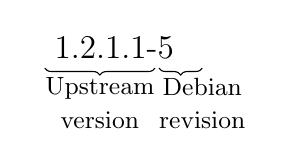
\begin{tikzpicture}
	    \draw (0,0) node[above right] {\large 1.2.1.1-5};
	    \draw [decorate,decoration={brace}] (2,0) -- (1.45,0) node[at start,below,text width=1.6cm,text centered] {\small  Debian revision};
	    \draw [decorate,decoration={brace}] (1.4,0) -- (0,0) node[midway,below,text width=1.6cm,text centered] { \small Upstream version};
\end{tikzpicture}
\end{center}


	  %%
  \item Edited manually or with \texttt{dch}
  \item Special format to automatically close Debian or Ubuntu bugs\\
    Debian: \texttt{Closes:~\#595268}; Ubuntu: \texttt{LP:~\#616929}
  \item Installed as \texttt{/usr/share/doc/\textit{package}/changelog.Debian.gz}
  \end{itemize}
  \seprule
  \begin{lstlisting}[basicstyle=\ttfamily\footnotesize]
hyphen-hi (0.6.0-1) unstable; urgency=low

  * Initial release (Closes: #542240) 

 -- Muneeb Shaikh <iammuneeb@gmail.com>  Sun, 31 Jul 2011 18:11:17 +0530
\end{lstlisting}
\end{frame}

\begin{frame}[fragile]{debian/control}
  \hbr
  \begin{itemize}
  \item Package metadata
    \begin{itemize}
    \item For the source package itself
    \item For each binary package built from this source
    \end{itemize}
    \hbr
  \item Package name, section, priority, maintainer, uploaders,
    build-dependencies, dependencies, description, homepage, \ldots \hbr
  \item Documentation: Debian Policy chapter 5\\
    \url{http://www.debian.org/doc/debian-policy/ch-controlfields.html}
  \end{itemize}

\end{frame}

\begin{frame}[fragile]{Sample debian/control}

\begin{lstlisting}[basicstyle=\fontsize{7pt}{10}\ttfamily]
Source: hyphen-hi
Section: text
Priority: optional
Maintainer: Muneeb Shaikh <iammuneeb@gmail.com>
Uploaders: Debian-IN Team <debian-in-workers@lists.alioth.debian.org>
Build-Depends: debhelper (>= 7.0.50~),
               dictionaries-common (>= 0.10)
Standards-Version: 3.9.2
Homepage: http://wiki.smc.org.in/Hyphenation
Vcs-Git: git://git.debian.org/debian-in/hyphen-hi.git
Vcs-Browser: http://git.debian.org/?p=debian-in/hyphen-hi.git;a=summary

Package: hyphen-hi
Architecture: all
Depends: ${misc:Depends},
         dictionaries-common (>= 0.10)
Recommends: libreoffice-writer | openoffice.org-writer
Description: Hindi hyphenation patterns for OpenOffice.org/LibreOffice
 Hyphenation is the process of inserting hyphens in between the syllables of
 a word so that when the text is justified, maximum space is utilized.
 .
 This package provides the hyphenation rules for Hindi language.

\end{lstlisting}
\end{frame}

\begin{frame}{Architecture: all or any}
  Two kinds of binary packages:
  \hbr
  \begin{itemize}
  \item Packages with different contents on each Debian architecture
    \begin{itemize}
    \item Example: C program
    \item \texttt{Architecture:\ any} in \texttt{debian/control}
      \begin{itemize}
      \item Or, if it only works on a subset of architectures:\\
        \texttt{Architecture:\ amd64 i386 ia64 hurd-i386}
      \end{itemize}
    \item buildd.debian.org: builds all the other architectures for you on upload
    \item Named \texttt{\textsl{package}\_\textsl{version}\_\textsl{architecture}.deb}
    \end{itemize}
    \br
  \item Packages with the same content on all architectures
    \begin{itemize}
    \item Example: Perl library
    \item \texttt{Architecture:\ all} in \texttt{debian/control}
    \item Named \texttt{\textsl{package}\_\textsl{version}\_\textbf{all}.deb}
    \end{itemize}
  \end{itemize}
  \br
  A source package can generate a mix of \texttt{Architecture:\ any} and \texttt{Architecture:\ all} binary packages
\end{frame}

\begin{frame}[fragile]{debian/rules}
  \hbr
  \begin{itemize}
  \item Makefile
    \br
  \item Interface used to build Debian packages
    \br
  \item Documented in Debian Policy, chapter 4.8\\
    {\small \texttt{http://www.debian.org/doc/debian-policy/ch-source.html\#s-debianrules}}
    \br
  \item Five required targets:
    \begin{itemize}
    \item \texttt{build}: should perform all the configuration and compilation
      \hbr
    \item \texttt{binary, binary-arch, binary-indep}: build the binary packages
      \begin{itemize}
      \item \texttt{dpkg-buildpackage} will call \texttt{binary} to build all
        the packages, or \texttt{binary-arch} to build only the
        \texttt{Architecture:~any} packages
      \end{itemize}
      \hbr
    \item \texttt{clean}: clean up the source directory
    \end{itemize}
  \end{itemize}
\end{frame}

\subsection{Build the package}

\begin{frame}[fragile]{Step 6: Build the package}
\hbr
\begin{itemize}
 \item Various tools to build the package.
 \begin{itemize}
  \item \textbf{dbkg-buildpackage}
  \item \textbf{debuild}
  \item \textbf{pdebuild}
  \item \textbf{git-buildpackage}
 \end{itemize}
 
 \item Execute following command to build the package. \newline
 \lstinline|$ dpkg-buildpackage -us -uc|
\end{itemize}

 \begin{lstlisting}[basicstyle=\fontsize{7pt}{10}\ttfamily]
  dpkg-buildpackage: export CFLAGS from dpkg-buildflags (origin: vendor): -g -O2
  dpkg-buildpackage: export CPPFLAGS from dpkg-buildflags (origin: vendor): 
  .
  .
  .
  dpkg-deb: building package `hyphen-hi' in `../hyphen-hi_0.7.0-2_all.deb'.
    dpkg-genchanges  >../hyphen-hi_0.7.0-2_amd64.changes
  dpkg-genchanges: not including original source code in upload
    dpkg-source --after-build hyphen-hi
  dpkg-buildpackage: binary and diff upload (original source NOT included)

 \end{lstlisting}
 
\end{frame}

\subsection{Check for errors}

\begin{frame}[fragile]{Step 6: Check for errors}
 \hbr
 \begin{itemize}
  \item Use \textbf{lintian} to check the errors and warnings in package.
  \begin{lstlisting}[basicstyle=\fontsize{10pt}{10}\ttfamily]
$ lintian hyphen-hi_0.7.0-2_amd64.changes 

W: hyphen-hi source: no-debian-copyright
E: hyphen-hi: no-copyright-file
  \end{lstlisting}

 \end{itemize}

\end{frame}


\subsection{Install the package}

\begin{frame}[fragile]{Step 7: Install the package}
  \hbr
 \begin{itemize}
  \item Use \textbf{dpkg} to install the package.
  \lstinline|$ sudo dpkg -i hyphen-hi_0.7.0-2_all.deb |

 \end{itemize}
   \begin{lstlisting}[basicstyle=\fontsize{8pt}{10}\ttfamily]
[sudo] password for muneeb: 
Selecting previously deselected package hyphen-hi.
(Reading database ... 602891 files and directories currently installed.)
Unpacking hyphen-hi (from hyphen-hi_0.7.0-2_all.deb) ...
Setting up hyphen-hi (0.7.0-2) ...
Processing triggers for postgresql-common ...
Building PostgreSQL dictionaries from installed myspell/hunspell packages...
  en_au
  en_ca
  en_gb
  en_us
  en_za

  \end{lstlisting}

\end{frame}

\subsection{Uploading to mentors.debian.net}

\begin{frame}[fragile]{Step 8: Uploading to mentors.debian.net}
 \hbr
  \begin{itemize}
    \item About \url{mentors.debian.net}
    \item Catch us on IRC or via email to know more about configuring it
    \begin{itemize}
     \item IRC: \textcolor{red}{\#debian-in-mentors} @ irc.oftc.net
     \item Mailing List: debian-in-workers
    \end{itemize}
  
  \item Upload the package using \texttt{dput}
  \lstinline|$ dput mentors-ftp hyphen-hi_0.7.0-2_amd64.changes|
  \end{itemize}

\end{frame}

\section{References}

\begin{frame}{References}
 \begin{itemize}
  \item Debian New Maintainers' Guide \\ \alert{\url{http://www.debian.org/doc/manuals/maint-guide/}}
  \item Packaging Tutorial \\ \alert{\url{http://wiki.debian.org/PackagingTutorial}}
  \item Intro to Debian Packaging \\ \alert{\url{http://wiki.debian.org/IntroDebianPackaging}}1
 \end{itemize}

\end{frame}

\begin{frame}
 \begin{center}
  {\Huge Queries?} \hbr \pause 
  {\Huge Thank You}
 \end{center}

\end{frame}


\end{document}
